\newcommand{\deriv}[3][]{% \deriv[<order>]{<func>}{<var>}
  \ensuremath{\frac{\partial^{#1} {#2}}{\partial {#3}^{#1}}}}

\chapter{A Dynamical Recipe for Cosmological Disks}\label{ch:background}

This chapter provides an overview of the background theory needed to understand subsequent chapters. In Chapter~\ref{ch:introduction}, we had a lot of discussion about simulations of galaxies being critical to having a theoretical understanding of cosmology and galaxy formation. The word ``simulation" was used without fully contextualizing its significance and meaning. We provide that context in \S\ref{sec:motivation}, where we describe what is actually being done when a simulation is run. In \S\ref{sec:galaxy_ics}, we talk about how to apply this theory to study the evolution of equilibrium galaxies. We also spoke at length about $\Lambda$CDM cosmology and how it is critical to explain the evolution of galaxies on a global scale. We talk about cosmology in detail in \S\ref{sec:cosmology}, and explain how this specifies an extended view of the discussion in \S\ref{sec:motivation}. Lastly, we talk about various techniques relied upon in the analysis of simulation in \S\ref{sec:analysis_of_sims}. This includes how we identify cosmic substructure and the techniques we use for analyzing the time-evolution of disk-derived quantities. This chapter summarizes the very basics of the models used in this thesis. It is by no means a comprehensive account of galactic dynamics. In the course of discussion, we will point the reader to more detailed accounts of the topics being discussed.

\section{Physical Motivation of Modeling} \label{sec:motivation}

The goal of this section is to convey to the reader what we mean by a simulation of a galactic system. 

\subsection{Thermodynamics of Self-Gravitating Systems}

The baryonic mass of the Milky Way is largely concentrated in its stars. To first order, the dynamical behavior of the Milky Way is determined by stellar material and dark matter \citep{BM}. While the evolution of gas is governed by the Euler equations with an equation of state, modelling in galactic dynamics requires that we understand how stars and dark matter behave. 

We begin by suggesting a model of a galaxy composed only of a very large number of stars and dark matter, where all stars have the same mass. We call the probability of a star being a specific position, $\textbf{r}$, and velocity $\textbf{v}$, at a time, $t$, the distribution function (DF), $f(\textbf{r},\textbf{v},t)$. The stars and dark matter sit in a combined gravitational potential, $\Phi(\textbf{r})$, in some near-equilibrium state. To fully describe this model, we need to understand how an ensemble of self-gravitating particles gives rise to an equilibrium distribution of stars and dark matter.

Unlike gas, which can exhange thermodynamic energy with itself through a variety of mechanisms, stars and dark matter interact only through gravity. Gravity is a long range force. In fact, the majority of the contribution to the forces on stars in galaxies comes from far outside their immediate neighborhoods (that is to say gravitational energy in non-extensive) \citep{BT}. 

This has a number of interesting implications. Classical equilibrium statistical mechanics tries to understand distributions of particles as ensembles with a given thermodynamic potential. Some commonly used ensembles are the microcanonical ensemble, where $f_0(\textbf{r},\textbf{v})$, the equilibrium state, is determined by holding energy fixed in a closed system, and the canonical ensemble which finds $f_0$ holding the temperature of the system fixed \citep{sethna}. These ensembles break down when non-extensive forces are involed (in the latter case, specifically because self-gravitating systems have no maximum entropy) \citep{self_gravitating_statistical_mechanics,lb_negative_specific_heat, BT}. Another peculiarity of self-gravitating systems is that they have a negative heat capacity \citep{lb_negative_specific_heat}.

The implication is that self-gravitating systems of stars, which have no means to dissipate internal energy, can never be in thermodynamic equilibrium. A system which starts in dynamical equilibrium evolves to a state of higher entropy when perturbed, which is physically characterized as having a dense core and extended envelope of mass \citep{BT}. Since a thermodynamic resolution of why galaxies evolve the way the do is unattainable due to the extensive nature of gravity, we are forced to study non-equilibrium dynamical evolution of $f(\textbf{r},\textbf{v},t)$ to understand galactic systems, and this requires more theory\footnote{For more information on the thermodynamics of self-gravitating systems, Chapter~4.10 of \citet{BT} and Chapter~7.3 of \citet{BT} provide excellent summaries.}.

\subsection{The Collisionless Boltzmann Equation}

To provide a time-dependent dynamical prescription for our model of stars and dark matter particles, we will make a number of assumptions that hold for the entire thesis. These are:

\begin{itemize}
\item Galaxies are collisionless systems; one does not have to worry about energy exchanged in close encounters because close encounters of individual stars and dark matter particles seldom happen.
\item All stars and dark matter particles are identical.
\item Phase space probability is conserved.
\item Phase space probability is incompressible.
\end{itemize}
We want to turn the assumptions listed above into a solvable equation for $f(\textbf{r},\textbf{v},t)$. This is done by recognizing that  for $\textbf{w} = (\textbf{p}, \textbf{q})$ \citep{BT},
\begin{equation}
\deriv{f}{t} + \deriv{}{\textbf{w}} \cdot \left( f \dot{\textbf{w}}\right) = 0
\end{equation}
is the continuity equation in 6D phase space that expresses conserved phase space probability. Here, $\textbf{p}$ and $\textbf{q}$ are any set of canonical coordinates. In general, this may be rewritten in what is commonly called the Collisionless Boltzmann equation (CBE),
\begin{equation}
\deriv{f}{t} + \dot{\textbf{q}} \cdot \deriv{f}{q} + \dot{\textbf{p}} \cdot \deriv{f}{p} = 0.
\end{equation}
The CBE is more commonly expressed in Cartesian coordinates as,
\begin{equation}
\deriv{f}{t} + \textbf{v} \cdot \deriv{f}{\textbf{x}} - \deriv{\Phi}{\textbf{x}} \cdot \deriv{f}{\textbf{v}} = 0, \label{eq:cbe_cartesian}
\end{equation}
where $\Phi$ is our total gravitational potential from stars and dark matter. The result is a quasilinear partial differential equation (PDE) for $f(\textbf{r},\textbf{v},t)$. The CBE is nothing more than an advection equation in phase space that expresses our view that particles are not self interacting, that they are identical, and that the phase space fluid is conserved and incompressible. In addition to the CBE which describes the evolution of the phase fluid, we have the Poisson equation, an elliptic equation describing the evolution of the potential \citep{BT},
\begin{equation}
\nabla^2 \Phi(\textbf{r},t) = -4 \pi G \rho(\textbf{r},t) \label{eq:poisson}
\end{equation} 
where $G$ is Newton's gravitational constant and,
\begin{equation}
\rho(\textbf{r},t) = \int_{\mathcal{D}} f(\textbf{r}, \textbf{v}, t) \text{d}^3 \textbf{v},
\end{equation}
where $\mathcal{D}$ is the phase space. We are left with a 6D space + 1D time solution domain on which to compute $f(\textbf{r},\textbf{v},t)$ as well as two PDEs and an integral.

\subsection{Monte Carlo Solution of the Collisionless Boltzmann Equation}

In terms of actually solving the CBE, we run into a number of technical challenges in applying traditional finite difference and finite volume schemes for advection equations. These techniques require that some mesh be constructed, and the flows between the cells in the mesh are calculated dependent on the type of equation being solved and the current states of the cells\footnote{Chapter~19 of \citet{numerical_recipes_fortran} discusses numerical methods for PDEs, although you could find detailed discussion of finite difference and finite volume methods in most numerical methods texts.}. The spatial domain is 6D, meaning a uniform mesh resolution scales in memory consuption as $O(N^6)$, where $N$ is the number of cells on an axis. For a sanity check, a modest $N = 2^5$ element grid would take up $2^{30} \times 2^4 \text{ bytes} \sim 17 \text{ GB}$. We obviously need more than 32 cells on an axis to represent the fine DF structure we want to study, and we are already at the limit of a single compute node to apply a finite difference scheme. 

This is where Monte Carlo methods shine. The fundamental principle on which they operate is that I can evaluate the integral of any function, $f(\textbf{x})$, over a domain $\mathcal{D}$, as \citep{numerical_recipes_fortran},
\begin{equation}
\int_\mathcal{D} f(\textbf{x}) d^{n} \textbf{x} = \frac{V(\mathcal{D})}{\vert X_s \vert} \sum_{\textbf{x}_i \in X_s(\mathcal{D})} f(\textbf{x}_i)
\end{equation}
where $X_s$ is a uniform random sample of points on $\mathcal{D}$, $V(\mathcal{D})$ is the volume of the domain, $n$ is the dimensionality of $\textbf{x}$, and $\vert X_s \vert$ is the cardinality, or number of points in the sample. The benefit of Monte Carlo integration is that although our result is not deterministic, the error in the integral is reduced as $1/\sqrt{N}$ \textit{regardless of the integral's dimension}! 

The point of introducing this powerful concept is simply in recognition of the fact that we need to integrate over phase space to solve Eq. \eqref{eq:cbe_cartesian}. As we stated, computing these integrals on a mesh is intractible, so we represent $f(\textbf{r},\textbf{v},t)$ in another way:
\begin{equation}
f(\textbf{r},\textbf{v},t) \approx \sum_i m_i \delta^3(\textbf{r} - \textbf{r}_i) \delta^3(\textbf{v} - \textbf{v}_i)
\end{equation}
where $\delta^3$ is the 3D Dirac delta function, and we take the DF to be normalized to $M = \sum_i m_i$ instead of 1. We call this the N-body realization of the DF. As an extension of this idea, to find $f(\textbf{r},\textbf{v},t)$ at some point in the future, it is sufficient to find the state of our \textit{approximation}\footnote{The author believes that this is one of the most beautiful results ever to be applied in studying the dynamics of galaxies.} at some time in the future. This requires a more detailed exploration of how we step through time with N-body realizations.

\subsection{Time Integration in N-Body Simulations}

We have shown how to map solving the CBE, the master equation for our system of stars and dark matter, to the evolution of a finite sample of particles. The system of equations we need to solve now is,
\begin{eqnarray} \label{eq:nbody_system}
\dot{\textbf{r}}_i(t) &=& \textbf{v}_i(t)\\
\dot{\textbf{v}}_i(t) &=& -\left.\deriv{\Phi}{\textbf{r}}\right\vert_{\textbf{r} = \textbf{r}_i}.
\end{eqnarray}
Our integro-differential equation system is now approximated as $6\,N$, where $N$ is the number of particles sampled to represent the stars and dark matter, ordinary differential equations (ODEs). These may be solved by any ODE system solver. There are two competing objectives when deciding on the best way to handle time stepping numerically; the first is that we want to maximize the accuracy of our integration scheme and the second is that we want to minimize the number of evaluations of $-\nabla \Phi$, the force. The latter consideration is a severe constraint because naively, the complexity of evaluating each pairwise force is $O(N^2)$.  Although, as we will see, approximations reduce this complexity to $O(N\,\log \, N)$. We note that finding the forces amounts to solving \eqref{eq:poisson}.

Nonetheless, the force calculation will be the most time consuming aspect of the integration, and we want to minimize the number of evaluations we need. This rules out some commonly used schemes in the Runge-Kutta class of integrators, since they would require four or five calculations of the force on millions of particles \citep{numerical_recipes_fortran}. The open question is how to construct a low-order integration scheme that preserves the Hamiltonian\footnote{In a collisionless system, the Hamiltonian should be conserved \citep{BT}.}.

Define the following drift and kick operators for a forward timestep of $\Delta t$ as \citep{quinn_1997},
\begin{eqnarray}
D_t(\Delta t) : \begin{cases} 
	  \textbf{r}_i & \longrightarrow  \textbf{r}_i + \textbf{v}_i \Delta t\\
      \textbf{v}_i & \longrightarrow  \textbf{v}_i 
   \end{cases},
\end{eqnarray}
and,
\begin{eqnarray}
K_t(\Delta t) : \begin{cases} 
	  \textbf{r}_i & \longrightarrow  \textbf{r}_i\\
      \textbf{v}_i & \longrightarrow  \textbf{v}_i  - \nabla \Phi(\textbf{r}_i) \Delta T
   \end{cases}.
\end{eqnarray}
If the Hamiltonian is separable as $\mathcal{H} = T(v) + V(r)$ for $T$, the kinetic energy, and  $V$, the potential energy, and we are in a Cartesian coordinate system, combinations of these operators approximately preserve the Hamiltonian. This is a property of a class of integrators known as symplectic integrators, whose derivation starts with an assumption of Hamiltonian mechanics. We use the second order scheme implemented in \textsc{Gadget-3}, based on the code in \citet{GadgetCodePaper}. This integration scheme is specified as,
\begin{equation}
U(\Delta T) = K(\frac{\Delta t}{2}) D(\Delta t) K(\frac{\Delta t}{2}).
\end{equation}
This integration scheme is reasonably accurate with only two force evaluations, and is colloquially referred to as Leapfrog. It is also symplectic, meaning that the Hamiltonian of the system will not drift. Chapter~3 of \citet{BT} has an excellent comparison of numerical integrators, including the Leapfrog scheme given here.

The final remaining complication for the timestepping portion of solving the CBE is determining the timesteps themselves. This is slightly more complicated to do properly than choosing a fixed timestep for all particles. This is because accelerations and velocities in astrophysical systems vary by orders of magnitude, and the timestep needs to be small compared to the timescales defined by the relevant accelerations. The way that this is commonly implemented, including in \citet{GadgetCodePaper}, is to have a base timestep for all particles that gets bisected at each level of refinement. That is to say, particles at level 4 are updated four more times than particles at level 2. Suppose the highest level of refinement is $k$. The simulation proceeds in $\Delta t_{base} / 2^{k}$ intervals, with particles at $k - 1$ being updated at half of the timesteps, dividing the number of updates by two up to the coarsest level of temporal refinement. Where multiple levels need updates, particles at the lower levels are updated first.

The level of temporal refinement assigned to a given particle is determined primarily by the acceleration it experiences. That is, for \textsc{Gadget-3} \citep{GadgetCodePaper},
\begin{equation}
\Delta t_i = \min\left(\Delta t_{base}, \left(\frac{2 \eta \epsilon}{\vert \nabla \Phi(\textbf{r}_i) \vert} \right)^{1/2}\right).
\end{equation}
Here, $\eta$ is a free accuracy parameter and $\epsilon$ is the gravitational softening. The gravitational softening is used to prevent numerical overflow when particles rarely have close encounters. It arises from having the acceleration induced from a particle at position $\textbf{r}_i$  be,
\begin{equation}
\textbf{a}_i(\textbf{r}) = -\frac{G m_i}{\left(\vert\textbf{r} - \textbf{r}_i\vert^2 + \epsilon^2\right)^{3/2}}(\textbf{r} - \textbf{r}_i) \label{eq:point_mass}
\end{equation}
Higher choices of $\epsilon$ reduce large errors accumulating due to unsustainably large forces, but also make the force calculation less accurate.

\subsection{Efficient Force Calculation}

The Leapfrog scheme requires us to compute the force two times. Naively, we would compute a sum over Eq. \eqref{eq:point_mass} for each of the $N(N-1)/2$ unique pairs of positions in $O(N^2)$ time to compute the forces on all particles. This is also intractible, or rather is the limiting factor on how large of a simulation we can run. Methods were developed early on in the history of running N-body simulations to cope with this by approximating the potential.

The first method worth noting for this thesis is the particle mesh technique \citep{hockney_pm, white_pm, klypin_pm}. This technique considers the calculation of forces on a 3D mesh by reducing the calculation to a Fast Fourier Transform (FFT) \citep{numerical_recipes_fortran}. One of the crowning achievements of scientific computing in the 20th century was the rediscovery of an algorithm by J. W. Cooley and John Tukey, originally discovered by Gauss, to compute the discrete fourier transform (DFT) in $O(N\,\log\,N)$ complexity\footnote{What Gauss was doing with recursive DFT algorithms is beyond the author, but in the author's humble opinion, it is expected from the greatest mathematician to ever live.}\citep{fft}. Particle mesh's cloud-in-cell (CIC) algorithm was a part of a flurry of algorithms that subsequently exploited the FFT. It has a difficult time accounting for forces from particles separated by small scales on the mesh, though \citep{GadgetCodePaper}.

Compensating for some of the shortcomings of the particle mesh approach, \citet{barnes_hut} introduced a new algorithm for approximating forces in $O(N \,\log\, N)$ complexity. Their algorithm took a divide an conquer approach by subdividing the simulation space into octants recursively until each particle was in its own cell. Forces would be computed pairwise for particles close together, but for distant particles, the mass distrubtion would be approximated as a multipole. To compute the forces, one simply does a depth-first-search (DFS) of the particle tree, going deeper if,
\begin{equation}
\frac{l}{d} \geq \theta
\end{equation}
where $l$ is the side length of the node whose force is being computed, $d$ is the distance from this node to the current node in the DFS, and $\theta$ is a threshold called the opening angle. In the simplest case, a cell not meeting this condition would be approximated as a point mass with the position at the  center of mass of all particles deeper in its subtree. Higher order multipole expansions are typically used (4 and 8 are common choices).

In addition, the somewhat simplistic opening angle scheme is expounded upon by some codes to include a ``relative opening criterion". The main idea is to use the last acceleration of the particle to determine whether or not a cell needs to be opened. \textsc{Gadget-3} uses the criterion,
\begin{equation}
\frac{G M}{d^2} \left(\frac{l}{d}\right)^2 \geq \alpha \vert\textbf{a}_{i,t-1} \vert
\end{equation}
where $M$ is the mass in the current DFS subtree, $\vert\textbf{a}_{i,t-1} \vert$ is the magnitude of the acceleration of the current particle at the last time step, and $\alpha$ is a relative opening criterion, a free parameter. Conceptually, this means that if the point mass acceleration in the current subtree is greater than a specified fraction of this particle's acceleration, the current DFS level is too coarse and we need to go deeper.

The scheme proposed by \citet{barnes_hut} is widely used in astrophysics because of its efficiency and computability. While both algorithms are $O(N\,\log\, N)$ complexity, tree-based methods tend to perform more slowly in practice \citep{GadgetCodePaper}. \citet{xu_treepm} introduced a scheme to combine both the short-range accuracy of tree methods with the efficiency of FFT-based methods. This TreePM method has been widely successful at handling short range forces with a tree method and long range forces with particle mesh techniques. The trick is forcing consistency between the two methods at intermediate distances. \textsc{Gadget-3} combines a high degree of optimization with the TreePM algorithm to produce a highly efficient algorithm.

Before proceeding to talk about the complications of executing TreePM on distributed systems like the Linux clusters worked with in this thesis, we would be remiss in not mentioning field expansion methods. Typically these take the form of an expansion of the potential in spherical harmonics using a set of radial basis functions. A brief discussion of these methods is presented in Chapter~2.9.4 of \citet{BT}. These methdos have great historical significance, and have even seen a recent resurgence in helping understand the structure of dark matter halos \citep{lilley_2018_a, lilley_2018_b}.

To summarize, there are a number of ways to find gravitational forces in a simulation that all amount to solving Poisson's Equation, \eqref{eq:poisson}. The most accurate way is to compute all pairwise forces, but efficient algorithms have been developed to accurately estimate forces from gravity. The force calculation together with a timestepping scheme for N-body realizations forms the main components of an N-body simulation, and solving Eq. \eqref{eq:nbody_system} to estimate $f(\textbf{r},\textbf{v},t)$ is what we mean when we say we ran a simulation.

\subsection{Complications on Distributed Systems}

\begin{figure}
	\centering
	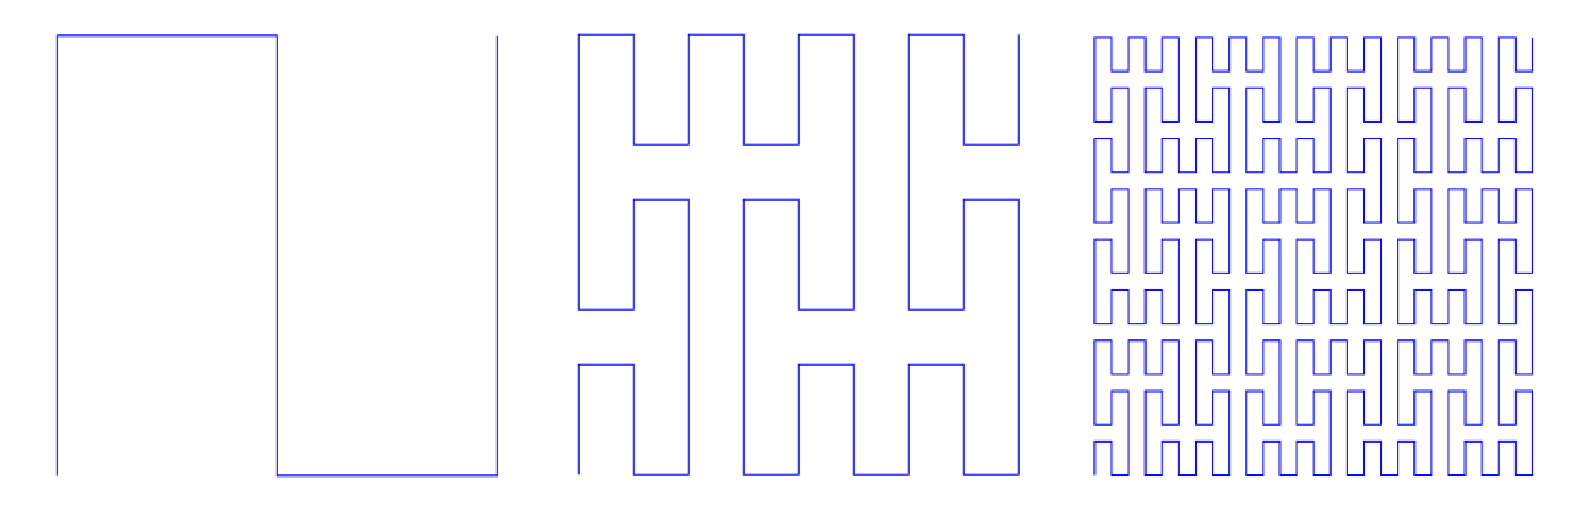
\includegraphics[width=\textwidth]{../figures/Peanocurve.eps}
	\caption{Several examples of the Peano space filling curve in 2D. The level of refinement increases left-to-right. Obtained from \citet{peano}.}\label{fig:peano}
\end{figure}

Modern high performance computing is largely done on compute clusters which are groups of smaller computers (nodes) connected with some high speed connection (Gigabit Ethernet, InfiniBand). The nodes form a distributed system in the sense that they do not share memory addresses. Each node may have multiple processes running (typically up to the number of logical cores on the node's CPU). Processes do not share data\footnote{Processes do not share data in a fully distributed model of parallel computing. Shared memory models like OpenMP \citep{openmp} share data between processes on a single node. MPI 3 even has similar shared memory support \citep{mpi3_shared}. \textsc{Gadget-3} was initially designed to not use these paradigms, and our intention is not to give a complete overview of all of parallel computing, so we relegate clarification to this footnote and references.}, and must communicate through a protocol like the Message Passing Interface (MPI) \citep{mpi_standard}.

Specifically, in an N-body simulation,  will have a subset of all of the particles, and a subset of the total tree structure. A naive DFS of an Octree simply cannot be done since no process will have all of the particles. When a process requires particles from another process, this reduces the efficiency gained from increasing the number of processors, and one might even get an overall slowdown. Another potential problem is that an individual process may get a higher work load than other processes, causing the other processes to wait for it to finish. We talk about how both of these problems are solved here.

To reduce the need to explicitly transfer particles between processes, \textsc{Gadget-3} notes that pairwise forces will only be needed for nearby poarticles. These represent the bulk of the tree force calculation. Any scheme which puts nearby particles on the same processor will reduce the overall communication time in the force calculation phase. One way to accomplish efficient load balancing is to partition the simulation space using a space filling curve. Fig. \ref{fig:peano} shows the Peano space-filling curve at several levels of refinement in 2D. This is the curve \textsc{Gadget-3} uses. A level of refinement is selected, and estimates of the computational cost in each cube are added up along the space filling curve to equally distribute the computational load. This results in nearby particles being on the same process, and in the processes having roughly equal work loads. \citet{GadgetCodePaper} shows that this is highly effective at reducing communication cost in the simulation, and it goes into more detail about how TreePM is carried out on distributed systems.


\section{Phase Space, Equilibrium, and Initial Conditions} \label{sec:galaxy_ics}
In \S\ref{sec:motivation} we outlined the underlying theory behind representing stars and dark matter in an N-body simulation. The focus of this thesis is studying the behavior of stellar disks in cosmological environments, and the first step towards that understanding is the construction of a pristine, equilibrium N-body model. Ultimately, in the course of running an N-body simulation, these pristine systems will diverge to higher entropy states, initially due to random errors in the N-body representation. Nonetheless, these models give us an understanding of how perfectly unperturbed galaxies will evolve due to the fact that real galaxies are also made of a finite number of particles.

\subsection{Jeans Modeling and the Epicyclic Approximation}

The DF represents the 6D phase space information and completely describes an N-body system. In a simple disk-halo system, there is a flattened axisymmetric component (the disk), and a spheroidal component (the dark matter halo) each with their own DF. These are made self-consistent by the separate DFs' incorporation of their combined gravitational potential. 

However, the DF is not the quantity that is observed in external galaxies. Astronomers are not typically working with a 6D phase space description of the structures they observe. Luminosity (density) profiles are one observable , as well as circular velocities (rotation curves) for disks, and also the spread of line of sight (LOS) velocties of disk stars. A modelling approach that takes our understanding of these observables as input is conceptually easier to understand than a DF which may or may not be unique \citep{BT}.

In this spirit, \citet{jeans_1915}\footnote{Notably before the infamous 1920 Curtis-Shapley debate \citep{curtis_shapley} establishing that so-called ``spiral nebulae" were actually external galaxies.} laid out a framework to describe galaxy evolution in terms of the \textit{moments} of the distribution function. Specifically, the idea is to multiply the CBE (Eq. \eqref{eq:cbe_cartesian}) by $\textbf{v}_i$ or $\textbf{v}_i \textbf{v}_j$ and integrate over the velocity part of phase space. These together yield the second-order Jeans equations \citep{BT},
\begin{eqnarray}
\deriv{\nu}{t} + \deriv{\nu \langle v_i \rangle}{x_i} &=& 0 \\
\nu \deriv{\langle v_j \rangle}{t} + \nu \langle v_i \rangle \deriv{\langle v_j \rangle}{x_i} &=& -\nu \deriv{\Phi}{x_j} - \deriv{\nu \sigma^2_{ij}}{x_i}\label{eq:jeans}
\end{eqnarray}
where $i,j \in (1,2,3)$, $\langle\cdot\rangle$ denotes expectation over $f$, $\mathbb{E}_f[\cdot]$, $\nu$ is the number density of particles, and $\sigma^2_{ij} = \langle v_i v_j \rangle - \langle v_i \rangle \langle v_j \rangle$ is the velocity dispersion tensor. In equilibrium for spherical systems, the second equation is often written as \citep{BT},
\begin{equation}
\deriv{\nu \langle v_r^2 \rangle}{r} + \nu \left(\deriv{\Phi}{r} + \frac{2 \langle v_r^2 \rangle - \langle v_\theta^2\rangle - \langle v_\phi^2 \rangle}{r} \right)
\end{equation}
where $\theta$ is the polar angle, $\phi$ is the azimuthal angle, and $r$ is the spherical radius\footnote{Note a slight abuse of notation. We said that $v_i$ has $i \in (1,2,3)$, but here we use symbols to represent specific coordinate systems. The point is that the indices have three unique values.}. Note that there is only one scalar equation. Symmetries in the velocity dispersion tensor for spherical systems require that the cross moments are zero \citep{BT}. For axisymmetric systems, the equilibrium Jeans equations are often written \citep{BT},
\begin{eqnarray}
\deriv{\nu \langle v_R^2 \rangle}{R} + \deriv{\nu \langle v_R v_z \rangle}{z} + \nu \left(\frac{\langle v_R^2 \rangle - \langle v_\phi^2 \rangle}{R} + \deriv{\Phi}{R} \right) &=& 0\\
\frac{1}{R} \deriv{R \nu \langle v_R v_z \rangle}{R} + \deriv{\nu \langle v_z^2 \rangle}{z}+ \nu \deriv{\Phi}{z} &=& 0\\
\frac{1}{R^2} \deriv{R^2 \nu \langle v_R v_\phi \rangle}{R} + \deriv{\nu \langle v_z v_\phi\rangle}{z} &=& 0
\end{eqnarray}
where $z$ is the Cartesian $z$, $R$ is the cylindrical radius, and $\phi$ is the polar angle. These equations look suspiciously like Euler's equations for fluid dynamics with a missing energy equation. \citet{jeans_1915} did not magically solve the statistical mechanical issues mentioned in \S\ref{sec:motivation}; given a number density and potential, we still have an unknown velocity dispersion tensor with six elements, and only 4 independent equations. In the simplified spherical case, we have three unknown elements and two independent equations.

We have also thrown out information about the DF by using moments and stopping at second order. Higher order Jeans equations can be appended to this system by multiplying the CBE by $v_i v_j v_k$ to obtain the third order equations, and so on. These get progressively more complicated, and we would require more additional equations to evaluate the equilibrium Jeans equations \citep{BT}.

Despite these shortcomings, more information can be imposed on the system to make these equations applicable. \citet{hernquist_1993} was one of the first successful applications of Jeans modelling to creating equilibrium galaxies with bulges, disks, and dark matter halos. In the case of the dark matter halo for a disk-halo system, one only has to specify the function,
\begin{equation}
\beta(r) = 1 - \frac{\langle v_\theta^2\rangle + \langle v_\phi^2 \rangle}{2 \langle v_R^2 \rangle}.
\end{equation}
This parameter measures anisotropy in the velocity ellipsoid defined by $\sigma_{ij}$ at each radius; $\beta = -\infty$ if all orbits are circular, $\beta=0$ if the system is isotropic, and $\beta = 1$ if orbits are purely radial. Together with an assumed density-potential pair, continuity equation, and the spherical second-order Jeans equation, the spherical halo's velocity structure is specified. At the time of writing, \citet{hernquist_1993} did not have much information about the dark matter distribution in galaxies (recall \citep{nfw} proceeded this work in establishing a common density profile for dark matter halos). As such, we will not talk about their uninformed choice of halo, and it really is not important.

In the case of the axisymmetric disk, \citet{hernquist_1993} based their model on the observations at the time which suggested that stellar disks had an exponential radial density profile \citep{freeman_1970}. This motivated a density profile commonly used today,
\begin{equation}
\rho_d(r) = \frac{M_d}{4 \pi R_d^2 h_d} e^{-R/R_d} \text{sech }^2\left(\frac{z}{z_d} \right). 
\end{equation}


% one has to specify a radial dispersion profile, which \citet{hernquist_1993} took to be,
\begin{equation}
\langle v_R^2 \rangle(R) = 
\end{equation}
\subsection{DF-based Models and the Strong Jeans Theorem}
\subsection{Action-Angle Variables}
\subsection{DFs as Functions of Actions}

\section{Cosmology and Implications for Galaxy Studies} \label{sec:cosmology}
\subsection{Basic FRW Cosmology}
\subsection{Extension of Numerical Methods}
\subsection{Sampling Initial Conditions for Cosmological Simulations}


\section{Simulation Analysis: Paradigms and Tools} \label{sec:analysis_of_sims}
\subsection{Cosmological Substructure and Halo Triaxiality}
\subsection{Identifying Substructure in Simulations}
\subsection{WKB Wave Analysis}
\subsection{Time Series Filtering}
\subsection{MCMC}
\bibliographystyle{apalike}
\bibliography{bibliography_background}


